\documentclass[../DC2017114Bouma.tex]{subfiles}
\begin{document}
\graphicspath{{01_Introduction/img/}}
\renewcommand{\chaptermark}[1]{\markboth{\thechapter.\ #1}{}}
\renewcommand{\sectionmark}[1]{\markright{#1}{}}
\cleartooddpage
\pagestyle{fancyreport}
\pagenumbering{arabic}

\chapter{Introduction}\label{ch:intro}
\section{High performance physical interaction in robotics}
In many applications of mechanical systems physical interaction with the environment is necessary to function, particularly in robotics. Humanoid robots, quadrupeds, and industrial robots are some examples of robots that repeatedly interact with their environment. Common control strategies that are available for these applications are limiting in performance. To avoid complexity of the controller, they often assume contact with their environment to happen at zero relative speed. This makes the robots less suitable for situations where speed is of significance, e.g., an industrial robot aiming to reach a certain throughput or a quadruped performing a trotting motion. Examples of such robots the SimLab quadruped \cite{VTquad} and the ABB IRB 360 flexpicker \cite{Flexpicker}, which are depicted in Figure~\ref{fig:1examples}. High performance is desirable in such cases, and zero velocity contact limits this performance. Therefore it is clear that the field of robotics can benefit from control strategies that are capable of handling non-zero relative velocity. Such controllers, however, are more complex than the controllers that require zero velocity contact situations.

\begin{figure}[b!]
\centering
\begin{subfigure}{0.48\textwidth}
\centering
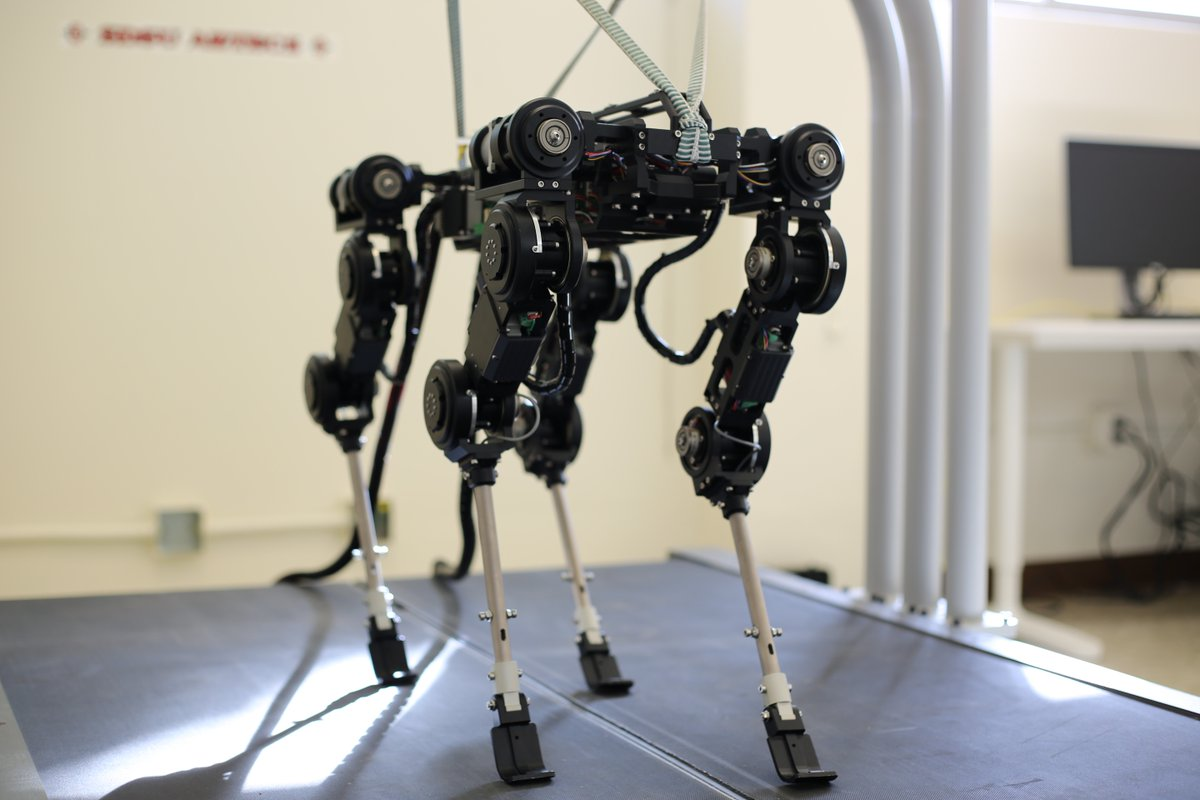
\includegraphics[width=\textwidth]{quadruped.jpg}\caption{SimLab quadruped used at Virginia Tech \cite{VTquad}.}\label{fig:quadrupedVT}
\end{subfigure}
\quad
\centering
\begin{subfigure}{0.48\textwidth}
\centering
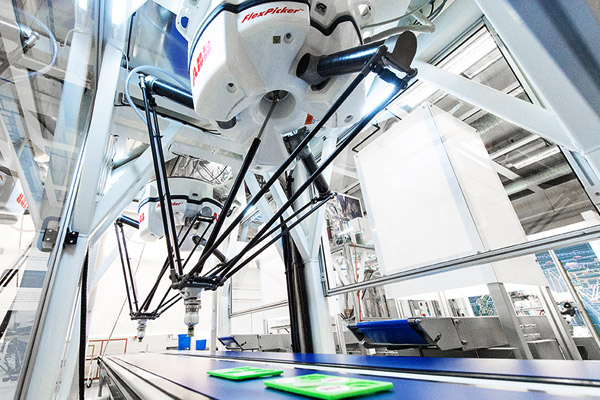
\includegraphics[width=\textwidth]{flexpicker.jpg}\caption{The ABB IRB 360 FlexPicker \cite{Flexpicker}.}\label{fig:flexpicker}
\end{subfigure}
\caption{Two examples of robots with physical interaction that can benefit from high performance control strategies.}\label{fig:1examples}
\end{figure}

When two bodies make physical contact at non-zero velocity, impact occurs. Impact is a complex physical event, that is characterized by dynamics at short timescales, high force levels, high energy dissipation rates, and large accelerations and decelerations. Due to the small time scale at which impacts happen, their effect is often modeled as instantaneous. In such a modeling setting, the contact forces are impulsive and the velocity experiences jumps during an impact. Such a modeling approach is pursued within \textit{nonsmooth mechanics}. Nonsmooth mechanical systems with impact are systems that have discontinuities in their state-evolution. In nonsmooth mechanics, a unilateral constraint is a constraint that prevents two bodies from penetrating. Mechanical systems with unilateral constraints are an example of systems that can exhibit nonsmooth behavior, as they experience velocity jumps when their unilateral constraints are closed at non-zero velocities. Control strategies for such systems are necessary to achieve higher performance.

\section{Nonsmooth modeling frameworks}
Nonsmooth systems can be described by several mathematical frameworks, e.g., singularly perturbed systems, hybrid systems, complementarity systems, and (measure-)differential inclusions \cite{Leine2004}. The singular perturbation framework approximates the nonsmooth behaviour using a singularly perturbed smooth system. In this way, the singularly perturbed system can be evaluated numerically using a single smooth differential equation. However, due to the smooth approximation the system becomes very stiff and needs extremely small time-steps in numerical simulation. 

More suitable for numerical evaluation are differential inclusions, which are applicable to systems with a discontinuous right-hand side but a time-continuous state-evolution (also called Filippov-systems \cite{Filippov1988}). A common example of Filippov-systems are systems experiencing dry friction. The differential inclusion gives a description of the nonsmooth dynamics in a single inclusion. However, mechanical systems with unilateral constraints and impact do not satisfy the requirement of having a time-continuous state-evolution. A measure-differential inclusion describes the continuous as well as the impulsive dynamics of a nonsmooth system \cite{Leine2008b}. In this way, measure-differential inclusions are suitable for systems with time-discontinuities in their state-evolution \cite{Moreau1988,Brogliato1999}. Using this approach, the dynamics can be accurately integrated using the timestepping method \cite{Wouwa}. 

From a control point-of-view the complementarity framework is often considered. This framework describes nonsmoothness through a combination of differential equations and inequalities \cite{VanDerSchaft1998,Heemels1999}. In \cite{Glocker2001}, the complementarity problem is used to describe mechanical systems with unilateral constraints. It plays a key role in mathematical programming, and several solutions for trajectory tracking using complementarity systems exist \cite{Bourgeot2005,Morarescu2010}. 

In recent years, the hybrid systems framework has drawn more interest for solving the trajectory tracking problem of nonsmooth systems \cite{Hyun2014,Morris2009}. A hybrid system is a dynamical system that exhibits both continuous and discrete dynamics behaviour, where it reinitializes the state and switches (discrete behaviour) between several differential equations (continuous behaviour) \cite{Goebel2009}. According to \cite{Ding2011a}, the hybrid systems framework is suitable for the modeling of mechanical systems with unilateral constraints as well as robotics. In a hybrid dynamical model guard sets are defined, which when entered by the state of the system, will cause the dynamics to switch from one differential equation to another and possibly reinitialize the state. This makes it a very intuitive approach to the modeling of nonsmoothness. 

A known difficulty with the hybrid system framework however, is a phenomenon called Zeno-behaviour. One speaks of Zeno-behaviour when an infinite amount of guard activations happen in a finite time. A classic example is the bouncing ball. Measure-differential inclusions with a timestepping scheme would be more suitable in such a situation, since the combined effect of several state resets is captured in a single time step. An advantage of using the hybrid systems framework, is that it is a more intuitive description of the dynamics whereas measure-differential inclusions are more abstract. The stability analyses for these frameworks are well-developed, i.e., \cite{Ye1998,Lygeros2003,Goebel2009} for hybrid systems, \cite{Pereira2004,Brogliato2004,Leine2008} for measure differential inclusions, and \cite{Brogliato1999,Camlibel2006,Camlibel2007} for linear complementarity problems.

\section{Tracking control for nonsmooth systems}
Legged robotic systems account for a substantial part of the research done into the trajectory tracking control of mechanical systems with unilateral constraints. Many results in this area deal with the stability of periodic orbits of systems with impacts. In \cite{Raibert1984}, a first big step has been made into modeling and controlling a one-legged hopping robot. In this research, the energy-loss during impact is modeled through damping and coupling effects are modeled as perturbations. Other pioneering works can be found in \cite{Lebaudy1993,Michalska1996,Gregorio1997}. 

In \cite{Grizzle2001,Morris2009}, the hybrid framework is adopted to find stable walking gaits for biped robots. Using Poincar\'{e} maps, the stability of periodic orbits with discontinuities of under-actuated systems are analyzed. Phases can be distinguished where the system is fully actuated and where the system is under-actuated. The fully actuated phase can then be used to stabilize the periodic trajectory despite the under-actuated phase. The work is continued in \cite{Ames2014}, generating control laws using data of walking humans and in \cite{Reher2016} the energy-efficiency of generated walking gaits has been the focus. An example of a humanoid robot on which such controllers have been implemented is Agility Robotics' Cassie \cite{Cassie}, which is depicted in Figure~\ref{fig:cassie}. An extensive survey in the field of bipedal robotic walking can be found in \cite{Grizzle2014}. The analysis of stable walking gaits is applied to the MIT Cheetah in \cite{Hyun2014}, where a stability analysis and controller design is presented for the trot-running of a quadrupedal robot.  

\begin{figure}[b!]
\centering
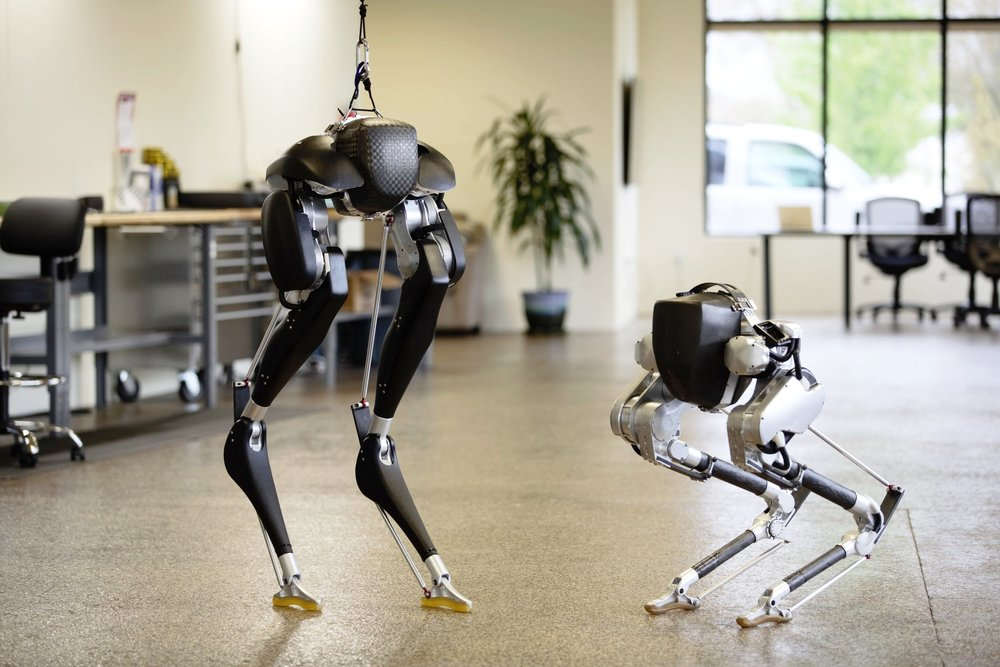
\includegraphics[width=.6\textwidth]{cassie.jpg}\caption{The bipedal robot Cassie developed by Agility Robotics \cite{Cassie}.}\label{fig:cassie}
\end{figure}

Considerable progress has been made in the field of walking robots and billiards, but it is easy to think of an example where nonperiodic trajectories are of interest. Under the assumption that the state trajectory jumps at the exact same time as the reference trajectory, the trajectory tracking problem for nonsmooth systems has been solved for several types of systems. The tracking problem for Lur'e type systems has been analyzed in \cite{VanDeWouw2008,Wouw2010}, using MDI's to describe nonsmooth and impulsive dynamics. The work uses the convergence property to provide a solution to the tracking problem, where the solution may be time-varying and exhibit state-jumps. In \cite{Bourgeot2005}, a passivity-based approach is used to solve the tracking control problem of complementarity Lagrangian systems. Asymptotic stability is achieved for Lagrangian systems with unilateral constraints. The same approach has been applied to the hybrid system framework in \cite{Naldi2013}, which results in a control law that can guarantee stability of a trajectory with multiple impacts. By embedding the reference trajectory with discontinuities into a set, Lyapunov tools can be used to analyze stability as in \cite{Sanfelice2011,Sanfelice2014}. In \cite{Posa2016} a stability analysis of systems with impacts and friction has been presented. The results are obtained using the measure-differential inclusion framework, resulting in a smooth control law. The planning and control of non-periodic bipedal locomotion with impacts and friction is discussed in \cite{Zhao2015a}.

In the prior discussed work, the tracking problem has been solved under the assumption that the jump of the state trajectory occurs at the same time-instant as the jump of the reference trajectory, i.e., in \cite{Naldi2013,Sanfelice2014,Posa2016}. In reality, especially in high velocity conditions, the time instant of the state jump and that of the reference trajectory jump are noncoincident more often than not. In this case a phenomenon called \textit{peaking} occurs \cite{Biemond2013}. Spikes in the tracking error will arise around the jump times, which generate large actuation forces and contradict stability.

Solutions to peaking of the tracking error exist for periodic orbits in \cite{Menini2001,Galeani2008}, where the results are compatible with a mismatch in reference jump-time and state jump-time for infinite time periodic trajectories with infinitely many state-jumps. Such trajectories are often found in so-called \textit{Birkhoff Billiards} where the coefficient of restitution is 1. \cite{Forni2013} also presents results for billiards, applicable to a large class of trajectories than \cite{Menini2001,Galeani2008}. In \cite{Biemond2013,Biemond2016}, a novel definition of the tracking error is introduced, using a distance function which is not sensitive to jumps of the state and the reference trajectory. Lyapunov-based conditions for the global asymptotic stability of non-smooth trajectories have been derived. Another solution for the problem of a jump-time mismatch is proposed in \cite{Baumann2018} in the form of a distance function similar to \cite{Biemond2013,Biemond2016} based on a quotient metric. When a state jump happens at a different time than the reference jump, this approach applies the jump map to the reference to be able to compare the state to the reference. In \cite{Kim2016}, a novel controller design using gluing functions is introduced to connect the start and end point of a jump in the state space. After gluing, the system can be considered a continuous or piecewise continuous function without state jumps. In \cite{Yang2017}, a tracking error is defined by taking the smallest of two values: the ante-impact tracking error and post-impact tracking error.

The solutions to the peaking behavior mentioned in the section above, do not always appear to be the best choice. It is beneficial to have some control over how the tracking error is defined, and particularly what the reference trajectory is, around the jump times. For this reason, a more intuitive and controllable solution to the peaking behavior is introduced.

\section{Reference spreading control}
In \cite{Saccon2014,Rijnen2015} a novel notion of error is introduced for systems with state jumps, by extending the reference trajectory segments, and considering the error between the reference trajectory and state trajectory that have encountered the same number of jumps. This way, an ante-event state trajectory can always be compared to an ante-event reference trajectory and a post-event state trajectory can always be compared to a post-event reference trajectory, even when the event times do not coincide. The extensions are defined by integrating the vector field, forwards and backwards, past the event times. This way, the input during the extension can be chosen in a particular way, to find a desired extension of the reference trajectory. These extensions will, comparable to the solutions presented in previous section, avoid peaking of the tracking error. The authors of \cite{Saccon2014,Rijnen2015} then use that notion of error as the basis for extending the sensitivity analysis introduced in \cite{Khalil1996} to the hybrid system framework. These results are then used to obtain a local approximation of the perturbed state dynamics. This analysis gives insight in how the system behaves under the presence of perturbations, which is useful for controller design. Experimental results for this control law are presented in \cite{Incremona2015}, where a 1-DOF robot arm performs an impacting trajectory using the control law proposed in \cite{Saccon2014}. In \cite{Rijnen2016}, a control strategy for hybrid systems with state triggered jumps is used on a hopping robotic leg model from \cite{Tsagarakis2013}. The control strategy is named \textit{reference spreading control} in \cite{Rijnen2017}, due to the extensions made on the reference trajectories in the notion of error. In \cite{Rijnen2017a}, the reference spreading control law is used in simulations with an iCub robot. The iCub robot balances on one foot and keeps himself standing upright by making and breaking contact with a wall using one of its arms. Some snapshots of the motion are depicted in Figure~\ref{fig:rijnen2017}. As mentioned earlier, many works in literature assume that the exact impact time is known. This is extremely limiting during implementation of the control law. Using the reference spreading approach, the impact time of the state is allowed to deviate from that of the reference, making implementation of the control law in practical applications more viable while still allowing for state-jumps.

\begin{figure}[bt!]
\centering
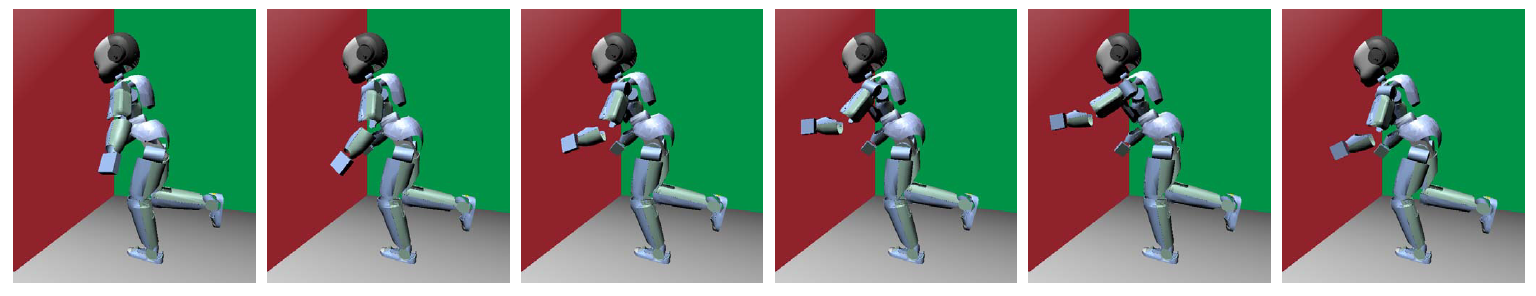
\includegraphics[width=\textwidth]{rijnen2017.PNG}\caption{Snapshots of the motion the iCub robot makes in the simulation done in \cite{Rijnen2017a} using reference spreading control.}\label{fig:rijnen2017}
\end{figure}

As is the case in the simulations with the iCub in Figure~\ref{fig:rijnen2017}, impacts are often modeled using a one-point contact between two bodies. However, in practice, more complex geometries can make contact with each other. The feet of Cassie in Figure~\ref{fig:cassie} for example, have a clear resemblance to human feet, which often results in distinct heel and toe strikes during walking motions. A more realistic contact geometry is used in \cite{Zhao2015}, in which the foot strike of a humanoid bipedal robot is modeled using multiple impacts. One strike is modeled by a heel impact, a toe impact, a heel release, and finally a toe release, resulting in a more realistic model of the walking gait of the bipedal robot. In such a movement, the order of impacts is known.

When considering a trajectory with multiple contacts closing at one time-instant, the problem becomes more complex. Imagine for example the iCub in \cite{Rijnen2017a} having a physically realistic geometry at the end of its arm. Consider Figure~\ref{fig:simultaneous}. The arm can first make a point contact, then a line contact, and finally a surface contact to make full contact with the wall. It can also track a trajectory where the surface of the arm makes a surface contact with the wall at one time-instant. Such events can be considered as multiple impacts happening at the same time-instant and are called \textit{simultaneous impacts}. One can imagine that a small perturbation can significantly change the behavior of a simultaneous impact. Instead of the expected single jump in the state, a perturbation can cause the state to have multiple jumps. Also the order of impacts of the several parts of the arm is not known beforehand. In Figure~\ref{fig:simultaneous} a 2-dimensional representation of the wrist of the iCub robot is illustrated. This image clearly visualizes the effect a perturbation has on a trajectory with simultaneous impacts. The approach used in \cite{Zhao2015} is not suitable for these situations.

\begin{figure}[hbt!]
\centering
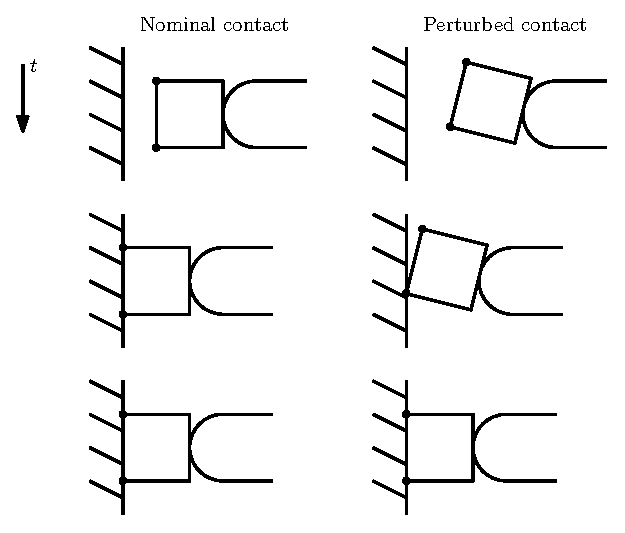
\includegraphics[width=.45\textwidth]{simultaneous.eps}\caption{A 2-dimensional illustration of the end effector of the wrist of the iCub robot. On the left: a nominal trajectory is illustrated (from top to bottom), where a simultaneous impact happens at the points indicated by black dots. The wrist immediately makes a line-contact with the surface. On the right: the trajectory is perturbed, which results in two subsequent impacts instead of one simultaneous impact.}\label{fig:simultaneous}
\end{figure}

The phenomenon of simultaneous impacts is first introduced in \cite{Chen2018a}, where the first step is taken into solving the trajectory tracking problem for such impacts. A hybrid system framework is used to model the impacts, where multiple guards can be activated at once. The reference spreading control in \cite{Rijnen2016,Rijnen2017} and the sensitivity analysis to approximate a system's behavior around trajectories with single guard activation, introduced in \cite{Saccon2014}, are extended to be suitable for simultaneous guard activation. The results of the sensitivity analyses are used to find a first-order approximation of the perturbed trajectory, which can be used to find suitable feedback gains. In addition to an impulse perpendicular to the impact-surface, taking friction into account will result in a tangential impulse. Also the release phase is not considered in \cite{Chen2018a}. During the release phase, no discontinuity in the state-evolution is seen, only a change in the number of active constraints on the system occurs. The aim of this research is to apply the reference spreading control strategy and sensitivity analysis to systems experiencing both impacts including friction and releasing motions.

\section{Research objectives and contribution}\label{sec:1resobj}
The research objective of this work is to extend the work presented in \cite{Rijnen2018a} in two ways: extending the sensitivity analysis to friction cases and release cases.
\subsection*{Simultaneous impacts with friction}
Friction elements are often disregarded when analyzing impacts. However, to set up a unifying theory, friction elements should not be ignored. Tangential impulses can have a considerable effect on a system's dynamics. Particularly for walking motions the frictional element of an impact is of importance. The impact laws used in the work of \cite{Chen2018a} can be extended using one of the several available friction laws \cite{Leine2008}. When impact laws are supplemented with a tangential element, this is often done using a Coulomb friction law \cite{Glocker2014a}. Besides the tangential impulse, also a Filippov-like discontinuity will be present due to Coulomb friction. Also in this work a Coulomb friction law will be used, which can lead to more accurate models and controllers for mechanical systems with unilateral constraints.\\\\
\textbf{Research Objective:}\\
\textit{Find a model suitable to describe mechanical systems with unilateral constraints and spatial friction. The sensitivity analysis and mathematical notation presented in \cite{Rijnen2018a} shall be extended to be compatible with such models.}

\subsection*{Simultaneous releases}
The release of two bodies is based on a force equilibrium. For this reason, the conditions that determine whether release happens is not only state dependent, but also input dependent. In \cite{Rijnen2016} and \cite{Rijn2016}, tracking of trajectories with events experiencing input-based triggers has been extensively researched. However, these results only include subsequent events. The release phase for simultaneous events is not yet investigated. In \cite{Chen2018a}, only the establishment of contact is simulated and release is not included. Extending the sensitivity analysis in \cite{Chen2018a} to be suitable for simultaneous releases would make it possible to simulate and control one trajectory with several simultaneous impacts and releases.\\\\
\textbf{Research Objective:}\\
\textit{Extending the sensitivity analysis presented in \cite{Rijnen2018a} such that it is suitable for input-triggered events.}


\section{Report outline}
The modeling of mechanical systems with unilateral constraints and spatial friction is discussed in Chapter~\ref{ch:model}. The generic dynamics of a mechanical system including contact and friction laws are derived, eventually resulting in a hybrid system with impulsive effects. Then, in Chapter~\ref{ch:order}, a tracking control strategy for hybrid systems with ordered state-input-triggered events is presented. In Chapter~\ref{ch:simult}, this tracking control strategy is extended to trajectories involving simultaneous impacts. An example of a mechanical system with unilateral constraints and spatial friction is given in Chapter~\ref{ch:vali}, which is used for a numerical validation of the presented control strategy. Finally, in Chapter~\ref{ch:concl}, conclusions are drawn and recommendations for future research are provided.

\end{document}